\section{Maximum likelihood estimation}
\label{sec:ch6:mle}

In studying network statistics, we often use single network models to represent random networks. These models are defined by certain key variables or parameters that shape the random networks they represent.

Suppose we encounter a real-world network and wish to understand it better. In doing so, we generally need to assume that this network is a specific sample of a random network characterized by certain parameters.

However, there's a catch here. This approach assumes that we already know these defining parameters, but that's not always the case. So, how do we handle this challenge?


\subsection{Erd\"os-R\'enyi (ER)}

Recall that the Erd\"os-R\'enyi (ER) random network has a single parameter: the probability of each edge existing, which we termed $p$. Thanks to the simplicity of the ER random network, we can use a method called Maximum Likelihood Estimation (MLE) to make an educated guess at what 'p' might be. For a deeper understanding of MLE, you can look at Appendix \ref{app:ch13:mle} and check out \cite{Casella2001Jun}.

Let's illustrate this concept with the familiar coin flip example.  Imagine you have a coin, but you don't know the probability of it landing on heads.  However, you're allowed to flip it 100 times and then guess the probability of it landing on heads. Let's say, after 100 flips, it landed on heads 45 times. What would be your guess for the probability of the coin landing on heads?

If you thought it might be $\frac{45}{100}$, or the number of heads you got divided by the total number of coin flips, you'd be right. This guess is the maximum likelihood estimate for a binary random variable.

The same principle applies to the ER random network. The best estimate of the probability of an edge existing in an ER random network is just the ratio of the total number of edges in the network, $m = \sum_{j > i}a_{ij}$, divided by the total number of edges possible in the network, which is $\binom n 2$.

Our result is:
\begin{align*}
    \hat p &= \frac{m}{\binom n 2}.
\end{align*}

The ``hat'' symbol ($\hat \cdot $) just means that $\hat p$ it is an \textit{estimator}: it is a function of the observed data that we use to describe the \textit{estimand}, which is the parameter of the model that we want to learn about. In this case, since we are considering an $ER_n(p)$ model, the only parameter that we want to learn about is $p$.

To bring this back to our coin flip example, this is like you are saying that there is a single coin. You flip the coin once for every possible edge between those pairs of communities, $\binom n 2$. When that coin lands on heads, that particular edge is determined to exist, and when it lands on tails, that edge does not exist. Our best guess, then, is just to count the number of heads you obtained, $m$, and divide by the number of coin flips you made, $\binom n 2$. 

Let's work on an example. You will use a sample of a random network which is ER, with $50$ nodes and an edge probability of $0.3$, similar to what we did in Section \ref{sec:ch5:er}. We begin by simulating and visualizing the appropriate network: 


\begin{lstlisting}[style=python]
from graspologic.simulations import er_np

p = 0.3
A = er_np(n=50, p=p)
\end{lstlisting}

Next, we'll fit the EREstimator model from \texttt{graspologic}, and compare the true probability $p=0.3$ to the estimated probability $\hat p$:
\begin{lstlisting}[style=python]
import numpy as np
from graspologic.models import EREstimator

model = EREstimator(directed=False, loops=False)
model.fit(A)
# obtain the estimate from the fit model
phat = model.p_
\end{lstlisting}

We can see how good the estimator performs by comparing it to the (true) population parameter, $p$:

\begin{lstlisting}[style=python]
print("Difference between phat and p: {:.3f}".format(phat - p))
\end{lstlisting}

Not bad! The estimate of the probability should end up pretty close to the true value. 

\subsection{Stochastic Block Model}

The Stochastic Block Model, like the Erdős-Rényi model, is characterized by a single parameter. However, in this case, the parameter is a block matrix, 'B'. The entries in $B$, $b_{kk'}$, denote the probabilities of edges existing between pairs of communities. 

When you apply the Maximum Likelihood Estimation (MLE) method to this model, you calculate $b_{kk'}$ by dividing $m_{kk'}$ by $n_{kk'}$. Here, $m_{kk'}$ stands for the total number of edges that actually exist between nodes in communities $k$ and $k$, while $n_{kk'}$ represents the total possible number of edges between these communities.

\begin{align*}
    \hat b_{kk'} = \frac{m_{kk'}}{n_{kk'}}.
\end{align*}

Intuitively, the estimate of the block probability $b_{kk'}$ is the ratio of how many edges you see between communities $k$ and $k'$ $m_{kk'}$ and how many edges were possible $n_{kk'}$.

To bring this back to our coin flip example, this is like saying that there is one coin $(k, k')$ for each pair of communities in our network. You flip each coin once for every possible edge between those pairs of communities, $n_{kk'}$. When that coin lands on heads, that edge exists, and when it lands on tails, that edge does not exist. Our best guess is just to count the number of heads we obtained, $m_{kk'}$, and divide by the number of coin flips we made, $n_{kk'}$. 

Remember that in the example we worked through in Section \ref{sec:ch5:sbm}, we had $100$ students, each of whom were in one of two schools (school $1$ and school $2$). If the students were both in school $1$, the probability that they were friends was $0.6$, and if the students were both in school $2$, the probability that they were friends was $0.4$. If the students attended different schools, the probability that they were friends was $0.2$. This gave us a block matrix of:
\begin{align*}
    B &= \begin{bmatrix}
        .6 & .2 \\
        .2 & .4
    \end{bmatrix}
\end{align*}

Which corresponds to a probability matrix $P$ where each entry is:
\begin{align*}
    p_{ij} &= \begin{cases}
    0.8 & i, j \leq 20 \text{ or }i, j \geq 20 \\
    0.2 & \text{otherwise}
    \end{cases}
\end{align*}

We begin by simulating an appropriate SBM:

\begin{lstlisting}[style=python]
from graspologic.simulations import sbm

n = [50, 50]
B = np.array([[0.6, 0.1], 
              [0.1, 0.4]])

A = sbm(n=n, p=B)
z = np.repeat([0, 1], repeats=[n1, n2])
\end{lstlisting}

A network sample is shown in Figure \ref{fig:ch5:sbm}.

Next, let's fit an appropriate SBM, and investigate the estimate of $B$:

\begin{lstlisting}[style=python]
from graspologic.models import SBMEstimator
from graphbook_code import heatmap

model = SBMEstimator(directed=False, loops=False)
model.fit(A, y=z)
Bhat = model.block_p_

# plot the block matrix vs estimate
heatmap(B, title=" $B$ true block matrix", vmin=0, vmax=1)
heatmap(Bhat, title="$\hat B$ estimate of block matrix", vmin=0, vmax=1)
heatmap(np.abs(Bhat - B), title="$|\hat B - B|$", vmin=0, vmax=1)
\end{lstlisting}

We investigate the difference between $B$ and $\hat B$ in Figure \ref{fig:ch6:sbm_est}.

\begin{figure}
    \centering
    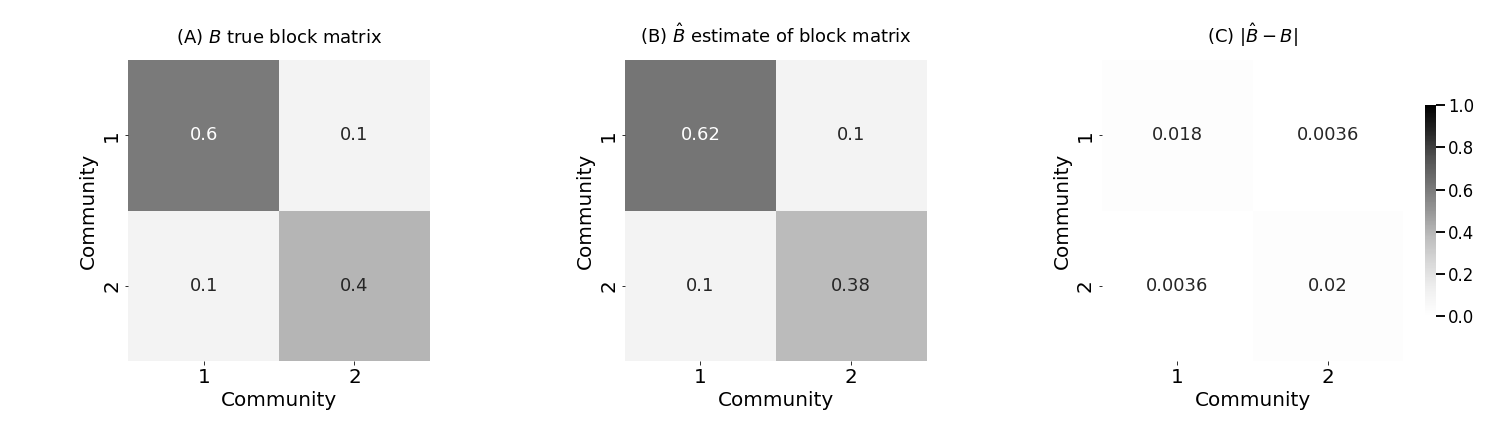
\includegraphics[width=\linewidth]{representations/ch6/Images/sbm_est.png}
    \caption[Estimating block matrix of SBM]{\textbf{(A)} the true block matrix underlying a random network. \textbf{(B)} the estimated block matrix from the network sample. \textbf{(C)} the difference between the estimated and true block matrices.}
    \label{fig:ch6:sbm_est}
\end{figure}

In this section, we've learned about estimating parameters for two types of simple networks. First, we have the $ER_n(p)$ random network. Here, edges are largely unstructured. Second, we have the $SBM_n(\vec z, B)$ network. For this, the network's structure is predetermined by known community assignments and we only need to understand 'B'.

For both types of random network, we can accurately estimate the underlying probability parameters of these models using methods like MLE.

These approaches allow us to make well-informed guesses about the likelihood of different types of connections within these networks.

\newpage